\documentclass[12pt,a4paper]{article}

% ── Packages ──────────────────────────────────────────────────────────────────
\usepackage[utf8]{inputenc}
\usepackage[T1]{fontenc}
\usepackage[english]{babel}
\usepackage{geometry}
\usepackage{graphicx}
\usepackage{hyperref}
\usepackage{listings}
\usepackage{xcolor}
\usepackage{amsmath}
\usepackage{amssymb}
\usepackage{booktabs}
\usepackage{longtable}
\usepackage{array}
\usepackage{multirow}
\usepackage{enumitem}
\usepackage{fancyhdr}
\usepackage{titlesec}
\usepackage{tcolorbox}
\usepackage{tikz}
\usepackage{pgfplots}
\usepackage{float}
\usepackage{caption}
\usepackage{subcaption}
\usepackage{setspace}
\usepackage{microtype}
\usepackage{lmodern}
\usepackage{mdframed}

\pgfplotsset{compat=1.18}
\usetikzlibrary{arrows.meta, positioning, shapes.geometric, fit, backgrounds}

% ── Page geometry ─────────────────────────────────────────────────────────────
\geometry{
  a4paper,
  top=2.5cm,
  bottom=2.5cm,
  left=3cm,
  right=2.5cm,
  headheight=15pt
}

% ── Colours ───────────────────────────────────────────────────────────────────
\definecolor{siriusblue}{RGB}{34,211,238}
\definecolor{siriuspurple}{RGB}{167,139,250}
\definecolor{critical}{RGB}{248,81,73}
\definecolor{high}{RGB}{240,136,62}
\definecolor{medium}{RGB}{210,153,34}
\definecolor{low}{RGB}{63,185,80}
\definecolor{codebg}{RGB}{13,17,23}
\definecolor{codegreen}{RGB}{126,231,135}
\definecolor{codekeyword}{RGB}{255,123,114}
\definecolor{codestring}{RGB}{166,227,161}
\definecolor{codecomment}{RGB}{100,116,139}
\definecolor{darkbg}{RGB}{22,27,34}

% ── Hyperref ──────────────────────────────────────────────────────────────────
\hypersetup{
  colorlinks=true,
  linkcolor=siriusblue,
  urlcolor=siriuspurple,
  citecolor=siriuspurple,
  pdftitle={SIRIUS AI -- Technical Report},
  pdfsubject={AI-Powered Security Incident Triage System},
}

% ── Code listings ─────────────────────────────────────────────────────────────
\lstdefinestyle{pythonstyle}{
  backgroundcolor=\color{codebg},
  basicstyle=\ttfamily\small\color{white},
  keywordstyle=\color{codekeyword}\bfseries,
  stringstyle=\color{codestring},
  commentstyle=\color{codecomment}\itshape,
  numberstyle=\tiny\color{codecomment},
  breaklines=true,
  breakatwhitespace=true,
  tabsize=4,
  showstringspaces=false,
  frame=single,
  framerule=0.5pt,
  rulecolor=\color{siriusblue!40},
  numbers=left,
  xleftmargin=1.5em,
  framexleftmargin=1.5em,
  captionpos=b,
}

\lstdefinestyle{yamlstyle}{
  backgroundcolor=\color{codebg},
  basicstyle=\ttfamily\small\color{white},
  keywordstyle=\color{siriusblue},
  stringstyle=\color{codestring},
  commentstyle=\color{codecomment}\itshape,
  breaklines=true,
  frame=single,
  framerule=0.5pt,
  rulecolor=\color{siriuspurple!40},
  showstringspaces=false,
  captionpos=b,
}

\lstdefinestyle{tsstyle}{
  backgroundcolor=\color{codebg},
  basicstyle=\ttfamily\small\color{white},
  keywordstyle=\color{codekeyword}\bfseries,
  stringstyle=\color{codestring},
  commentstyle=\color{codecomment}\itshape,
  breaklines=true,
  frame=single,
  framerule=0.5pt,
  rulecolor=\color{siriuspurple!40},
  showstringspaces=false,
  captionpos=b,
}

% ── Section formatting ────────────────────────────────────────────────────────
\titleformat{\section}{\Large\bfseries\color{siriusblue}}{\thesection}{1em}{}[\color{siriusblue!30}\hrule]
\titleformat{\subsection}{\large\bfseries\color{siriuspurple}}{\thesubsection}{1em}{}
\titleformat{\subsubsection}{\normalsize\bfseries}{\thesubsubsection}{1em}{}

% ── Header / footer ───────────────────────────────────────────────────────────
\pagestyle{fancy}
\fancyhf{}
\fancyhead[L]{\small\color{gray}SIRIUS AI --- Technical Report}
\fancyhead[R]{\small\color{gray}AI-Powered Security Incident Triage}
\fancyfoot[C]{\small\color{gray}\thepage}
\renewcommand{\headrulewidth}{0.4pt}
\renewcommand{\footrulewidth}{0.4pt}

% ── Custom boxes ──────────────────────────────────────────────────────────────
\tcbuselibrary{skins,breakable}

\newtcolorbox{infobox}[1][]{
  colback=siriusblue!5,
  colframe=siriusblue!50,
  fonttitle=\bfseries,
  #1
}

\newtcolorbox{techbox}[1][]{
  colback=darkbg,
  colframe=siriuspurple!50,
  fonttitle=\bfseries\color{siriuspurple},
  coltitle=siriuspurple,
  #1
}

% ── Document ─────────────────────────────────────────────────────────────────
\begin{document}

% ── Title page ────────────────────────────────────────────────────────────────
\begin{titlepage}
  \centering
  \vspace*{1.5cm}

  {\Huge\bfseries\color{siriusblue} SIRIUS AI}\\[0.5em]
  {\Large\color{siriuspurple} AI-Powered Security Incident Triage Assistant}\\[0.3em]
  {\large\color{gray} Comprehensive Technical Report}

  \vspace{1.5cm}

  
\begin{tikzpicture}
    \foreach \r in {2.8,2.6,2.4}{
      \draw[siriusblue!\the\numexpr 40\relax, line width=\r*0.4pt, opacity=0.4] (0,0) circle (\r cm);
    }
    \draw[siriusblue, line width=2pt] (0,0) circle (2.2cm);
    \draw[siriuspurple, line width=1.5pt] (0,0) circle (1.5cm);
    \filldraw[siriusblue!20] (0,0) circle (0.8cm);
    \node at (0,0) {\huge\bfseries\color{siriusblue}S};
    \foreach \angle in {0,45,90,135,180,225,270,315}{
      \draw[siriusblue!60, line width=1pt] (\angle:2.2cm) -- (\angle:2.5cm);
    }
  \end{tikzpicture}

  \vspace{1.5cm}

  \begin{tabular}{rl}
    \textbf{Version}    & 2.0.0 \\[0.3em]
    \textbf{Date}       & May 2026 \\[0.3em]
    \textbf{Backend}    & FastAPI 0.115 + Python 3.13 \\[0.3em]
    \textbf{Frontend}   & React 19 + TypeScript (strict) \\[0.3em]
    \textbf{Repository} & \href{https://github.com/Karyaustuncelik/AI-Powered-Security-Incident-Triage-Assistant}{github.com/Karyaustuncelik} \\[0.3em]
    \textbf{License}    & MIT \\
  \end{tabular}

  \vfill

  \begin{mdframed}[linecolor=siriusblue!40, backgroundcolor=siriusblue!5]
    \centering
    \small\color{gray}
    This document provides a complete technical specification of the SIRIUS AI platform,\\
    covering system architecture, security engineering modules, AI/ML subsystems,\\
    API design, and frontend implementation.
  \end{mdframed}

\end{titlepage}

% ── ToC ───────────────────────────────────────────────────────────────────────
\tableofcontents
\newpage

% =============================================================================
\section{Executive Summary}
% =============================================================================

SIRIUS AI is a full-stack, production-grade security operations platform that combines
artificial intelligence, statistical analysis, and real-time network reconnaissance to
deliver enterprise-level incident triage capabilities. The system is designed to reduce
mean time to detect (MTTD) and mean time to respond (MTTR) for security operations centre
(SOC) analysts by automating the most labour-intensive aspects of incident investigation.

\begin{infobox}[title=Platform Highlights]
\begin{itemize}[noitemsep]
  \item \textbf{ReAct-pattern autonomous security agent} with 8 real network tools
  \item \textbf{Detection Engineering Panel}: SIGMA rules $\rightarrow$ Splunk SPL / Microsoft Sentinel KQL
  \item \textbf{Statistical anomaly detection} using z-score across 5 behavioural dimensions
  \item \textbf{Compliance mapping} to NIST CSF 2.0, CIS Controls v8, OWASP Top 10 2021, ISO 27001:2022
  \item \textbf{MITRE ATT\&CK} technique tagging for every detection rule
  \item \textbf{Automated penetration testing} workflow with CVE correlation via NIST NVD
  \item \textbf{Real-time streaming} via Server-Sent Events (SSE) throughout the platform
  \item \textbf{Glassmorphism UI} with live attack map, kill-chain builder, threat intelligence feed
\end{itemize}
\end{infobox}

The backend exposes \textbf{16 REST/SSE API endpoints} across a layered FastAPI application,
while the frontend delivers \textbf{8 distinct pages} rendered as a single-page application (SPA)
in React 19 with TypeScript strict mode.

\subsection{Codebase Metrics}

\begin{table}[H]
\centering
\caption{Codebase size by component}
\begin{tabular}{lrr}
\toprule
\textbf{Component} & \textbf{Files} & \textbf{Lines of Code} \\
\midrule
Backend services (Python)     & 18 & $\approx$ 4{,}800 \\
Backend API routes (Python)   & 11 & $\approx$ 900 \\
Backend models \& utils       &  8 & $\approx$ 600 \\
Frontend components (TSX)     & 22 & $\approx$ 5{,}200 \\
Frontend styles (CSS)         & 14 & $\approx$ 3{,}100 \\
\midrule
\textbf{Total}                & \textbf{73} & $\approx$ \textbf{14{,}600} \\
\bottomrule
\end{tabular}
\end{table}

% =============================================================================
\section{System Architecture}
% =============================================================================

\subsection{High-Level Overview}

The platform follows a clean three-tier architecture with clear separation of concerns.
The React SPA communicates with the FastAPI backend exclusively over HTTP/SSE; no WebSocket
connections are required. The backend is composed of a thin routing layer, a rich service
layer, and a lightweight data layer built on JSON files and SQLite.

\begin{figure}[H]
\centering
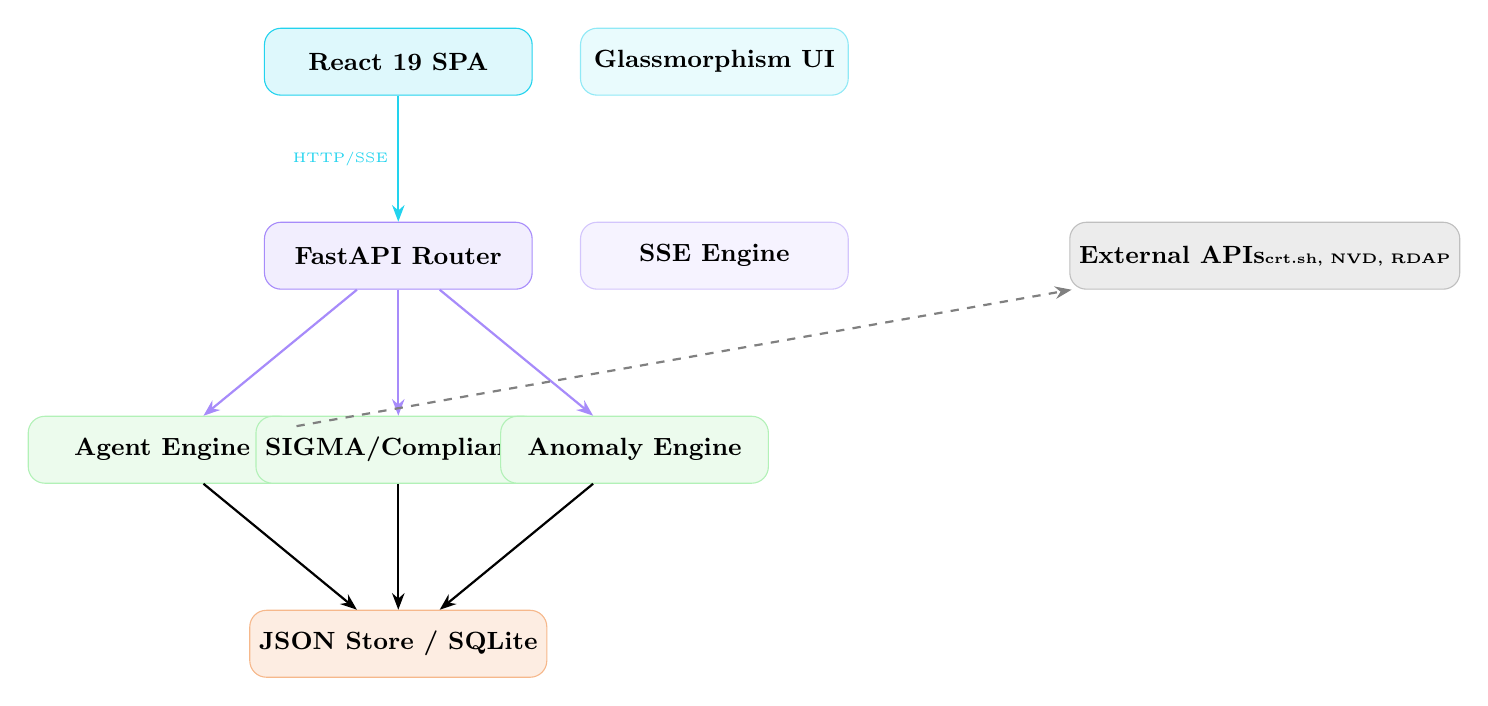
\begin{tikzpicture}[
  box/.style={rectangle, rounded corners=6pt, draw, minimum width=3.4cm,
              minimum height=0.85cm, font=\small\bfseries, text centered},
  arrow/.style={-{Stealth[length=6pt]}, thick}
]
% Tier 1: Presentation
\node[box, fill=siriusblue!15, draw=siriusblue] (spa) {React 19 SPA};
\node[box, fill=siriusblue!10, draw=siriusblue!50, right=0.6cm of spa] (css) {Glassmorphism UI};

% Tier 2: Application
\node[box, fill=siriuspurple!15, draw=siriuspurple, below=1.6cm of spa] (api) {FastAPI Router};
\node[box, fill=siriuspurple!10, draw=siriuspurple!50, right=0.6cm of api] (sse) {SSE Engine};

% Tier 3: Services
\node[box, fill=codegreen!15, draw=codegreen!60,
      below=1.6cm of api, xshift=-3cm] (agent) {Agent Engine};
\node[box, fill=codegreen!15, draw=codegreen!60,
      below=1.6cm of api] (sigma) {SIGMA/Compliance};
\node[box, fill=codegreen!15, draw=codegreen!60,
      below=1.6cm of api, xshift=3cm] (anomaly) {Anomaly Engine};

% Tier 4: Data
\node[box, fill=high!15, draw=high!60,
      below=1.6cm of sigma] (data) {JSON Store / SQLite};

% External
\node[box, fill=gray!15, draw=gray!50,
      right=2.8cm of sse] (ext) {External APIs\\{\tiny crt.sh, NVD, RDAP}};

% Arrows
\draw[arrow, siriusblue] (spa) -- node[left, font=\tiny]{HTTP/SSE} (api);
\draw[arrow, siriuspurple] (api) -- (agent);
\draw[arrow, siriuspurple] (api) -- (sigma);
\draw[arrow, siriuspurple] (api) -- (anomaly);
\draw[arrow] (agent) -- (data);
\draw[arrow] (sigma) -- (data);
\draw[arrow] (anomaly) -- (data);
\draw[arrow, dashed, gray] (agent) -- (ext);
\end{tikzpicture}
\caption{High-level three-tier system architecture}
\end{figure}

\subsection{Technology Stack}

\begin{table}[H]
\centering
\caption{Technology stack summary}
\begin{tabular}{lll}
\toprule
\textbf{Layer} & \textbf{Technology} & \textbf{Notes} \\
\midrule
\multirow{4}{*}{Backend}
  & Python 3.13          & Type-annotated throughout \\
  & FastAPI $\geq$0.115  & Async ASGI framework \\
  & Uvicorn              & Production-ready ASGI server \\
  & Pydantic v2          & Data validation, serialisation \\
\midrule
\multirow{4}{*}{Frontend}
  & React 19             & Latest concurrent features \\
  & TypeScript           & Strict mode, zero \texttt{any} \\
  & Vite                 & Sub-second HMR dev server \\
  & CSS3                 & Custom properties, \texttt{backdrop-filter} \\
\midrule
\multirow{3}{*}{Data}
  & JSON files           & $\approx$200 synthetic incidents \\
  & SQLite               & Pentest session persistence \\
  & In-memory            & Baseline caches, upload sessions \\
\midrule
\multirow{4}{*}{External}
  & NIST NVD API v2      & Live CVE database queries \\
  & crt.sh API           & Certificate Transparency subdomains \\
  & RDAP (rdap.org)      & Domain registration lookups \\
  & Python \texttt{ssl}  & Native TLS handshake analysis \\
\bottomrule
\end{tabular}
\end{table}

\subsection{Project Directory Structure}

\begin{lstlisting}[style=pythonstyle, caption=Annotated project directory tree]
siber+llm/
|-- backend/
|   |-- app/
|   |   |-- api/routes/           # 11 route modules
|   |   |   |-- agent.py          # POST /agent/run  (SSE stream)
|   |   |   |-- sigma.py          # Detection engineering endpoints
|   |   |   |-- pentest.py        # Pentest session workflow
|   |   |   |-- incidents.py      # Incident queue + detail
|   |   |   `-- ...               # health, stats, uploads, review, etc.
|   |   |-- models/
|   |   |   `-- domain.py         # 30+ Pydantic models
|   |   |-- services/
|   |   |   |-- agent/
|   |   |   |   |-- tools.py      # 8 security tools  (564 LOC)
|   |   |   |   `-- engine.py     # ReAct loop        (523 LOC)
|   |   |   |-- sigma_service.py       # SIGMA generator  (327 LOC)
|   |   |   |-- anomaly_service.py     # z-score engine   (308 LOC)
|   |   |   |-- compliance_service.py  # Framework mapper (224 LOC)
|   |   |   `-- pentest_service.py     # Pentest workflow (1230 LOC)
|   |   `-- core/config.py
|   `-- requirements.txt
`-- frontend/
    `-- src/
        |-- components/
        |   |-- nebula/            # Glassmorphism page components
        |   |   |-- AgentWorkspace.tsx
        |   |   |-- AttackMap.tsx
        |   |   |-- KillChainBuilder.tsx
        |   |   |-- NebulaCopilot.tsx
        |   |   `-- ThreatIntel.tsx
        |   |-- DetectionPanel.tsx
        |   `-- PentestWorkspace.tsx
        |-- api/                   # Typed API clients
        |-- types/                 # TypeScript interfaces
        `-- App.tsx                # SPA router (8 routes)
\end{lstlisting}

% =============================================================================
\section{Backend Architecture}
% =============================================================================

\subsection{Application Factory Pattern}

The backend uses the \emph{application factory pattern} to instantiate the FastAPI application.
This separates configuration from execution and simplifies both testing and future multi-environment
deployment:

\begin{lstlisting}[style=pythonstyle, caption=Application factory in main.py (simplified)]
def create_app() -> FastAPI:
    settings = get_settings()
    app = FastAPI(title=settings.app_name, version="0.1.0")
    app.add_middleware(
        CORSMiddleware,
        allow_origins=["http://localhost:5173"],
        allow_credentials=True,
        allow_methods=["*"],
        allow_headers=["*"],
    )
    for router in [health_router, explain_router, incidents_router,
                   uploads_router, review_router, stats_router,
                   red_team_router, pentest_router,
                   agent_router, sigma_router]:
        app.include_router(router)
    return app

app = create_app()
\end{lstlisting}

\subsection{Domain Model Hierarchy}

The system uses Pydantic v2 for all data contracts. The complete model graph is shown below:

\begin{figure}[H]
\centering
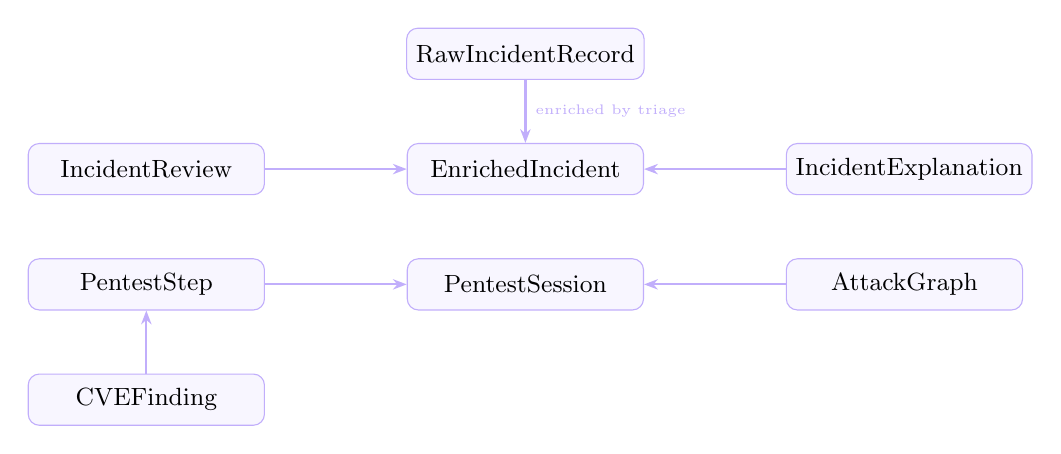
\begin{tikzpicture}[
  model/.style={rectangle, rounded corners=4pt, draw=siriuspurple!70,
                fill=siriuspurple!8, minimum width=3cm, minimum height=0.65cm,
                font=\small, text centered},
  arrow/.style={-{Stealth[length=5pt]}, siriuspurple!70, thick}
]
\node[model] (raw)      {RawIncidentRecord};
\node[model, below=0.8cm of raw]     (enr)  {EnrichedIncident};
\node[model, left=1.8cm of enr]      (rev)  {IncidentReview};
\node[model, right=1.8cm of enr]     (exp)  {IncidentExplanation};
\node[model, below=0.8cm of enr]     (sess) {PentestSession};
\node[model, left=1.8cm of sess]     (step) {PentestStep};
\node[model, right=1.8cm of sess]    (ag)   {AttackGraph};
\node[model, below=0.8cm of step]    (cve)  {CVEFinding};

\draw[arrow] (raw) -- node[right,font=\tiny]{enriched by triage} (enr);
\draw[arrow] (rev) -- (enr);
\draw[arrow] (exp) -- (enr);
\draw[arrow] (step) -- (sess);
\draw[arrow] (ag) -- (sess);
\draw[arrow] (cve) -- (step);
\end{tikzpicture}
\caption{Core Pydantic model relationships}
\end{figure}

\subsection{Severity and Priority Levels}

\begin{table}[H]
\centering
\caption{Severity level definitions and response SLA}
\begin{tabular}{llll}
\toprule
\textbf{Severity} & \textbf{Score Range} & \textbf{Priority} & \textbf{Response SLA} \\
\midrule
CRITICAL & 85--100 & Immediate attention & $<$ 15 minutes \\
HIGH     & 65--84  & Investigate soon   & $<$ 1 hour \\
MEDIUM   & 40--64  & Investigate soon   & Same day \\
LOW      & 0--39   & Investigate later  & Next business day \\
\bottomrule
\end{tabular}
\end{table}

\subsection{Complete API Endpoint Catalogue}

\begin{longtable}{lllp{5.5cm}}
\caption{All API endpoints exposed by the platform}\\
\toprule
\textbf{Method} & \textbf{Path} & \textbf{Type} & \textbf{Description} \\
\midrule
\endfirsthead
\multicolumn{4}{c}{\small\itshape (continued)} \\
\toprule
\textbf{Method} & \textbf{Path} & \textbf{Type} & \textbf{Description} \\
\midrule
\endhead
\bottomrule
\endfoot
GET  & \texttt{/health}                   & REST & Liveness check \\
GET  & \texttt{/incidents}                & REST & Paginated incident list with filters \\
GET  & \texttt{/incidents/\{id\}}         & REST & Enriched incident detail \\
GET  & \texttt{/incidents/\{id\}/explain} & SSE  & LLM narrative explanation stream \\
GET  & \texttt{/stats}                    & REST & Dashboard KPI aggregations \\
GET  & \texttt{/filters}                  & REST & Available filter option lists \\
POST & \texttt{/uploads}                  & REST & Log file upload, parse, correlate \\
GET  & \texttt{/uploads/\{id\}}           & REST & Upload session detail \\
POST & \texttt{/review/\{id\}}            & REST & Analyst review submission \\
POST & \texttt{/pentest/sessions}         & REST & Create new pentest session \\
POST & \texttt{/pentest/sessions/\{id\}/step} & SSE & Stream next pentest step analysis \\
\textbf{POST} & \texttt{\textbf{/agent/run}}  & \textbf{SSE} & \textbf{Autonomous security agent} \\
GET  & \texttt{/agent/tools}              & REST & Available agent tool schemas \\
GET  & \texttt{/detection/sigma/\{id\}}   & REST & SIGMA rule generation \\
GET  & \texttt{/detection/compliance/\{id\}} & REST & Compliance framework mapping \\
GET  & \texttt{/detection/anomaly/\{id\}} & REST & Anomaly z-score report \\
\end{longtable}

% =============================================================================
\section{AI Security Agent --- ReAct Engine}
% =============================================================================

\subsection{ReAct Pattern}

The agent implements the \textbf{ReAct} (Reasoning + Acting) paradigm, a state-of-the-art
agentic design pattern where a language model alternates between producing a chain-of-thought
and executing tool invocations:

\begin{equation}
\text{Agent Loop} = \bigl(\text{Thought} \to \text{Action} \to \text{Observation}\bigr)^{*} \to \text{Final Answer}
\end{equation}

\begin{figure}[H]
\centering
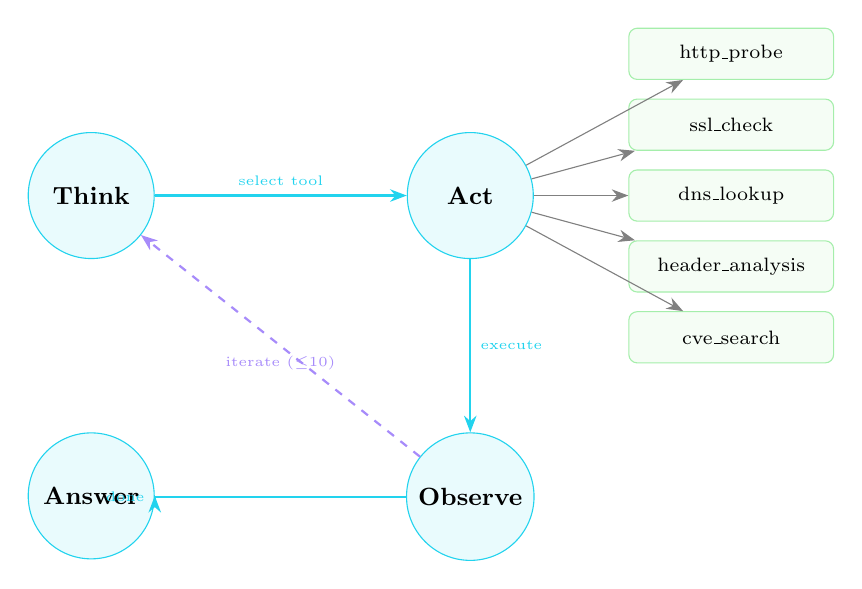
\begin{tikzpicture}[
  state/.style={circle, draw=siriusblue, fill=siriusblue!10,
                minimum size=1.6cm, font=\small\bfseries},
  tool/.style={rectangle, rounded corners=3pt, draw=codegreen!70, fill=codegreen!8,
               minimum width=2.6cm, minimum height=0.65cm, font=\scriptsize, text centered},
  arrow/.style={-{Stealth[length=6pt]}, thick}
]
\node[state] (T)  {Think};
\node[state, right=3.2cm of T] (A) {Act};
\node[state, below=2.2cm of A] (O) {Observe};
\node[state, below=2.2cm of T] (F) {Answer};

\draw[arrow, siriusblue] (T) -- node[above,font=\tiny]{select tool} (A);
\draw[arrow, siriusblue] (A) -- node[right,font=\tiny]{execute} (O);
\draw[arrow, siriuspurple, dashed] (O) -- node[below,font=\tiny]{iterate ($\leq$10)} (T);
\draw[arrow, siriusblue] (O.west) -| node[left,font=\tiny, near end]{done} (F.east);

\node[tool, right=1.2cm of A, yshift= 1.8cm] (t1) {http\_probe};
\node[tool, right=1.2cm of A, yshift= 0.9cm] (t2) {ssl\_check};
\node[tool, right=1.2cm of A, yshift= 0.0cm] (t3) {dns\_lookup};
\node[tool, right=1.2cm of A, yshift=-0.9cm] (t4) {header\_analysis};
\node[tool, right=1.2cm of A, yshift=-1.8cm] (t5) {cve\_search};

\foreach \t in {t1,t2,t3,t4,t5}
  \draw[arrow, gray, thin] (A) -- (\t);
\end{tikzpicture}
\caption{ReAct agent loop with tool dispatch}
\end{figure}

\subsection{Agent Tool Catalogue}

\begin{table}[H]
\centering
\caption{Security agent tools --- all make real network requests}
\begin{tabular}{llp{7.5cm}}
\toprule
\textbf{Tool} & \textbf{Protocol} & \textbf{Capabilities} \\
\midrule
\texttt{http\_probe}      & HTTP/S & Status code, Server/X-Powered-By headers, technology fingerprinting via body signatures (React, Angular, Vue, WordPress, Django, Laravel, ASP.NET, \ldots{}), form count \\[4pt]
\texttt{header\_analysis} & HTTP/S & OWASP header grading A+$\to$F: CSP, HSTS, X-Frame-Options, X-Content-Type-Options, Referrer-Policy, Permissions-Policy with individual penalty scoring \\[4pt]
\texttt{dns\_lookup}      & DNS    & A/AAAA records via \texttt{socket.getaddrinfo}, reverse DNS \\[4pt]
\texttt{ssl\_check}       & TLS    & Certificate CN/SAN, validity dates, expiry warnings ($<$30 d), cipher suite enumeration via native Python \texttt{ssl} module \\[4pt]
\texttt{subdomain\_enum}  & HTTPS  & Certificate Transparency enumeration via \texttt{crt.sh} JSON API (passive, no DNS brute-force) \\[4pt]
\texttt{path\_discovery}  & HTTP/S & 30 common sensitive paths: \texttt{/.env}, \texttt{/.git/HEAD}, \texttt{/admin}, \texttt{/swagger}, \texttt{/actuator}, \texttt{/phpinfo.php}, \texttt{/wp-config.php}, \ldots{} \\[4pt]
\texttt{cve\_search}      & HTTPS  & NIST NVD REST API v2 --- real CVE data with CVSS v3 scores, sorted by severity \\[4pt]
\texttt{whois\_lookup}    & HTTPS  & RDAP domain registration via \texttt{rdap.org} \\
\bottomrule
\end{tabular}
\end{table}

\subsection{Execution Modes}

The engine supports two modes, selected automatically at runtime:

\begin{enumerate}
  \item \textbf{LLM-powered mode.} When \texttt{OPENAI\_API\_KEY} is set, the engine uses
        OpenAI-compatible function-calling to let the model choose tools dynamically, producing
        contextual reasoning for each step. The loop runs for up to 10 iterations.

  \item \textbf{Deterministic fallback.} When no LLM is configured, a fully deterministic
        pipeline executes all 7 tools in a fixed sequence, guaranteeing a complete security
        report with zero external LLM dependency. This makes the agent useful in air-gapped
        or offline environments.
\end{enumerate}

\subsection{SSE Event Stream Schema}

Results are pushed to the browser in real time via Server-Sent Events:

\begin{lstlisting}[style=pythonstyle, caption=SSE event types and payload shapes]
# Every event frame:  data: <JSON>\n\n

{ "type": "thought",    "content": "Analysing TLS configuration..." }
{ "type": "tool_call",  "tool": "ssl_check", "params": {...},
                        "description": "Inspecting TLS certificate" }
{ "type": "tool_result","observation": "{\"cert_cn\": \"example.com\",...}" }
{ "type": "finding",    "severity": "HIGH",
                        "title": "Missing HSTS header",
                        "category": "header", "description": "...",
                        "recommendation": "...", "evidence": "..." }
{ "type": "progress",   "step": 3, "total": 7 }
{ "type": "summary",    "overall_risk": "HIGH",
                        "findings_count": 5, "text": "..." }
{ "type": "done" }
\end{lstlisting}

\subsection{Finding Severity Classification}

\begin{table}[H]
\centering
\caption{Finding severity criteria per tool}
\begin{tabular}{llp{7cm}}
\toprule
\textbf{Severity} & \textbf{Colour Code} & \textbf{Example Conditions} \\
\midrule
CRITICAL & \textcolor{critical}{$\blacksquare$} Red    & \texttt{/.env} accessible (credential exposure), expired SSL certificate, CVSS $\geq$ 9.0 \\
HIGH     & \textcolor{high}{$\blacksquare$} Orange  & \texttt{/.git/HEAD} readable, missing HSTS, CVSS 7.0--8.9 \\
MEDIUM   & \textcolor{medium}{$\blacksquare$} Yellow & Missing CSP header, SSL expiry $<$ 30 days, wildcard subdomain cert \\
LOW      & \textcolor{low}{$\blacksquare$} Green   & Missing Referrer-Policy, informational path responses \\
INFO     & $\blacksquare$ Blue   & Technology stack fingerprint, RDAP data, DNS records \\
\bottomrule
\end{tabular}
\end{table}

% =============================================================================
\section{Detection Engineering}
% =============================================================================

\subsection{SIGMA Rule Generator}

SIGMA is the industry-standard, vendor-agnostic signature format for SIEM detection rules.
SIRIUS AI's \texttt{SigmaRuleGenerator} converts any enriched incident into a fully-formed
SIGMA YAML rule and then compiles it to two platform-specific query languages.

\subsubsection{MITRE ATT\&CK Technique Mapping}

Every generated rule is automatically tagged with the corresponding ATT\&CK techniques,
enabling direct integration with the MITRE Navigator:

\begin{table}[H]
\centering
\caption{Incident event type to MITRE ATT\&CK mapping}
\begin{tabular}{lll}
\toprule
\textbf{Incident Event Type} & \textbf{Technique ID} & \textbf{Tactic} \\
\midrule
\texttt{multiple\_failed\_login\_attempts}  & T1110, T1110.001 & Credential Access \\
\texttt{repeated\_authentication\_failures} & T1110             & Credential Access \\
\texttt{risky\_sign\_in\_pattern}           & T1078, T1078.004 & Defense Evasion / Initial Access \\
\texttt{impossible\_travel\_pattern}        & T1078, T1550      & Initial Access / Lateral Movement \\
\texttt{unusual\_privilege\_escalation}     & T1078.002, T1098 & Privilege Escalation / Persistence \\
\texttt{suspicious\_api\_activity}          & T1106, T1059.009 & Execution \\
\texttt{abnormal\_access\_outside\_hours}   & T1078             & Persistence \\
\bottomrule
\end{tabular}
\end{table}

\subsubsection{Generated SIGMA Rule Example}

\begin{lstlisting}[style=yamlstyle, caption=Sample SIGMA rule --- brute-force detection]
title: "Brute Force Login Detection"
id: "a1b2c3d4-e5f6-7890-abcd-ef1234567890"
status: experimental
description: >
  Multiple consecutive failed authentication attempts from
  the same actor -- potential brute force attack.
author: SIRIUS AI Detection Engine
date: 2026-05-18
tags:
  - attack.credential_access
  - attack.t1110
  - attack.t1110.001
logsource:
  category: authentication
  product: azure_signin
  service: azure_ad
detection:
  selection:
    ActorUpn|contains: "user@example.com"
    ResultType: "50074"
  condition: selection | count() by ActorUpn > 10
  timeframe: 15m
level: high
falsepositives:
  - Legitimate forgotten passwords
  - Password managers re-syncing
\end{lstlisting}

\subsubsection{Multi-Platform Compilation}

\begin{figure}[H]
\centering
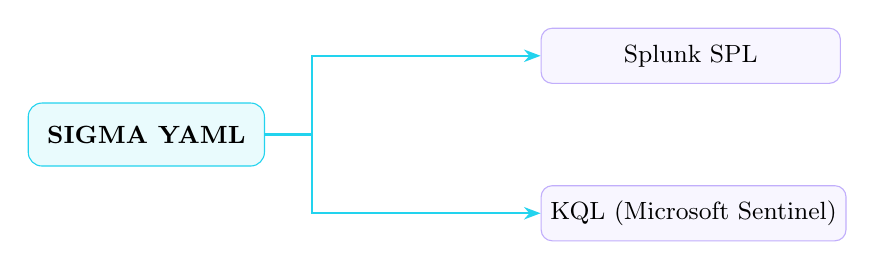
\begin{tikzpicture}[
  src/.style={rectangle, rounded corners=5pt, draw=siriusblue, fill=siriusblue!10,
              minimum width=3cm, minimum height=0.8cm, font=\small\bfseries},
  dst/.style={rectangle, rounded corners=4pt, draw=siriuspurple!70, fill=siriuspurple!8,
              minimum width=3.8cm, minimum height=0.7cm, font=\small, text centered},
  arrow/.style={-{Stealth[length=6pt]}, thick, siriusblue}
]
\node[src] (sigma) {SIGMA YAML};
\node[dst, right=3.5cm of sigma, yshift= 1.0cm] (splunk) {Splunk SPL};
\node[dst, right=3.5cm of sigma, yshift=-1.0cm] (kql)    {KQL (Microsoft Sentinel)};

\draw[arrow] (sigma.east) -- ++(0.6,0) |- (splunk.west);
\draw[arrow] (sigma.east) -- ++(0.6,0) |- (kql.west);
\end{tikzpicture}
\caption{SIGMA rule multi-platform compilation}
\end{figure}

\subsection{Compliance Framework Mapper}

The \texttt{ComplianceMapper} maps any incident to four compliance frameworks simultaneously.
Each mapping includes a relevance grade (High / Medium / Low) and a human-readable description
linking the incident context to the control requirement.

\begin{table}[H]
\centering
\caption{Supported compliance frameworks and covered controls}
\begin{tabular}{llll}
\toprule
\textbf{Framework} & \textbf{Version} & \textbf{Controls} & \textbf{Focus} \\
\midrule
NIST CSF    & 2.0  & PR.AA, DE.CM, RS.MA, ID.AM & Identity \& Access Management \\
CIS Controls & v8   & 5, 6, 8, 13, 14, 16        & Endpoint, IAM, Network \\
OWASP Top 10 & 2021 & A01--A07                   & Web Application Security \\
ISO 27001   & 2022 & A.5, A.8, A.9, A.10        & Information Security ISMS \\
\bottomrule
\end{tabular}
\end{table}

% =============================================================================
\section{Statistical Anomaly Detection Engine}
% =============================================================================

\subsection{Mathematical Foundation}

The anomaly detector applies the classical z-score formula to measure how far an observed
metric deviates from a user's historical behavioural baseline:

\begin{equation}
z = \frac{x - \mu}{\sigma}
\label{eq:zscore}
\end{equation}

\noindent where $x$ is the observed metric value, $\mu$ is the running mean for that
user/entity, and $\sigma$ is the running standard deviation.

\begin{table}[H]
\centering
\caption{Z-score interpretation thresholds}
\begin{tabular}{cclc}
\toprule
\textbf{$|z|$ range} & \textbf{Percentile} & \textbf{Classification} & \textbf{Alert?} \\
\midrule
$< 2.0$           & $<$ 95th  & Normal         & No \\
$2.0 \leq z < 3.0$ & 95th--99.7th & Anomaly   & Flag \\
$\geq 3.0$        & $>$ 99.7th & Strong Anomaly & Immediate \\
\bottomrule
\end{tabular}
\end{table}

\subsection{Five Behavioural Dimensions}

\begin{enumerate}
  \item \textbf{Login Frequency} --- authentication event count vs.\ historical window
  \item \textbf{API Volume} --- API request count vs.\ user's baseline average
  \item \textbf{Privilege Changes} --- permission change count vs.\ baseline frequency
  \item \textbf{Geographic Diversity} --- distinct countries in session vs.\ typical geo-spread
  \item \textbf{Time Anomaly} --- after-hours activity ratio vs.\ user's schedule pattern
\end{enumerate}

\subsection{Composite Score (RMS)}

Individual z-scores are aggregated into a single composite score using root mean square,
which is more sensitive to multiple simultaneous anomalies than a simple average:

\begin{equation}
z_{\text{composite}} = \sqrt{\frac{1}{N} \sum_{i=1}^{N} z_i^{2}}
\label{eq:rms}
\end{equation}

\subsection{Risk Multiplier}

A non-linear risk multiplier escalates the composite score for strong anomalies:

\begin{equation}
M =
\begin{cases}
  1.50 & z_{\text{composite}} \geq 3.0 \\
  1.25 & 2.0 \leq z_{\text{composite}} < 3.0 \\
  1.10 & 1.5 \leq z_{\text{composite}} < 2.0 \\
  1.00 & \text{otherwise}
\end{cases}
\label{eq:multiplier}
\end{equation}

\begin{figure}[H]
\centering
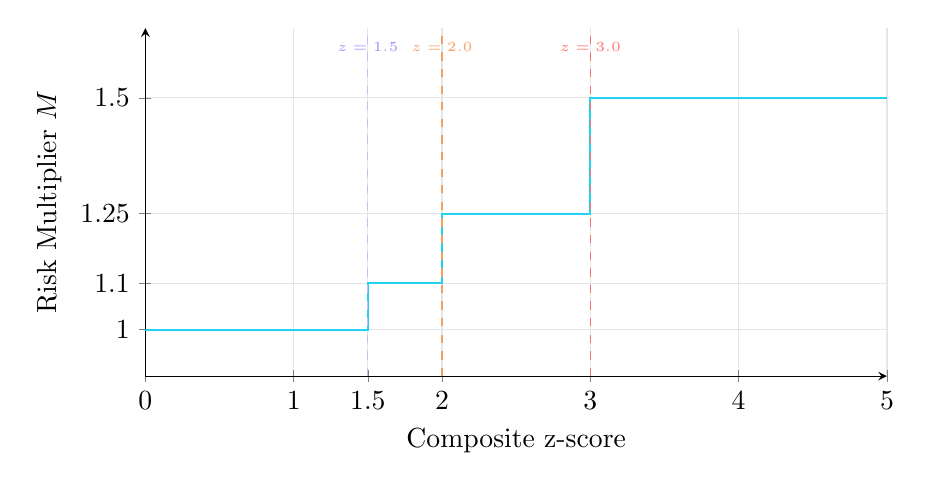
\begin{tikzpicture}
\begin{axis}[
  width=11cm, height=6cm,
  xlabel={Composite z-score},
  ylabel={Risk Multiplier $M$},
  xmin=0, xmax=5,
  ymin=0.90, ymax=1.65,
  grid=both, grid style={gray!20},
  axis lines=left,
  xtick={0,1,1.5,2,3,4,5},
  ytick={1.00,1.10,1.25,1.50},
]
\addplot[siriusblue, thick, const plot] coordinates {
  (0,1.00)(1.5,1.00)(1.5,1.10)(2.0,1.10)(2.0,1.25)(3.0,1.25)(3.0,1.50)(5,1.50)
};
\addplot[siriuspurple!60, dashed, thin] coordinates {(1.5,0.90)(1.5,1.65)};
\addplot[high!80,          dashed, thin] coordinates {(2.0,0.90)(2.0,1.65)};
\addplot[critical!80,      dashed, thin] coordinates {(3.0,0.90)(3.0,1.65)};
\node[font=\tiny,siriuspurple] at (axis cs:1.5,1.61) {$z=1.5$};
\node[font=\tiny,high!80]      at (axis cs:2.0,1.61) {$z=2.0$};
\node[font=\tiny,critical!80]  at (axis cs:3.0,1.61) {$z=3.0$};
\end{axis}
\end{tikzpicture}
\caption{Risk multiplier as a step function of composite z-score}
\end{figure}

\subsection{Deterministic Baseline Simulation}

For reproducibility in the portfolio build, baselines are generated deterministically
using a hash of the user ID and metric name. The same user/metric pair always produces
the same $(\mu, \sigma)$ pair:

\begin{lstlisting}[style=pythonstyle, caption=Deterministic baseline generation]
def _simulate_baseline(self, user_id: str, metric: str
                       ) -> tuple[float, float]:
    seed = hash(f"{user_id}:{metric}") % 10_000
    mean = 5.0 + (seed % 50) / 10.0
    std  = max(1.0 + (seed % 20) / 20.0, 0.5)
    return mean, std
\end{lstlisting}

% =============================================================================
\section{Penetration Testing Workflow}
% =============================================================================

\subsection{Session Lifecycle}

\begin{figure}[H]
\centering
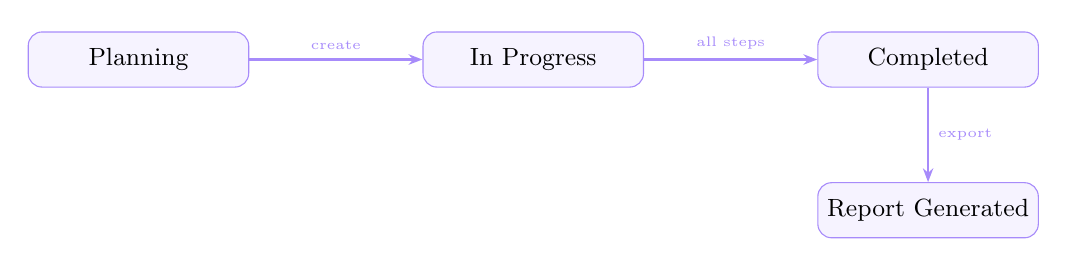
\begin{tikzpicture}[
  state/.style={rectangle, rounded corners=5pt, draw=siriuspurple, fill=siriuspurple!10,
                minimum width=2.8cm, minimum height=0.7cm, font=\small, text centered},
  arrow/.style={-{Stealth[length=5pt]}, siriuspurple, thick}
]
\node[state] (plan) {Planning};
\node[state, right=2.2cm of plan] (run)  {In Progress};
\node[state, right=2.2cm of run]  (done) {Completed};
\node[state, below=1.2cm of done] (rep)  {Report Generated};

\draw[arrow] (plan) -- node[above,font=\tiny]{create} (run);
\draw[arrow] (run)  -- node[above,font=\tiny]{all steps} (done);
\draw[arrow] (done) -- node[right,font=\tiny]{export} (rep);
\end{tikzpicture}
\caption{Pentest session lifecycle}
\end{figure}

\subsection{Pentest Steps}

Each session is decomposed into six structured phases:

\begin{table}[H]
\centering
\caption{Pentest session phases}
\begin{tabular}{cll}
\toprule
\textbf{Phase} & \textbf{Title} & \textbf{Outputs} \\
\midrule
1 & Reconnaissance       & WHOIS, DNS, subdomains, cert info \\
2 & Enumeration          & Open services, versions, tech stack \\
3 & Vulnerability Analysis & CVE matches from NIST NVD \\
4 & Exploitation (Simulated) & Attack path mapping \\
5 & Post-Exploitation    & Persistence \& lateral movement paths \\
6 & Reporting            & Severity-graded findings \\
\bottomrule
\end{tabular}
\end{table}

\subsection{Attack Graph Model}

The \texttt{AttackGraph} is a directed graph with typed nodes and edges:

\begin{table}[H]
\centering
\caption{Attack graph node and status types}
\begin{tabular}{lll}
\toprule
\textbf{Node Type} & \textbf{Represents} & \textbf{Status Options} \\
\midrule
\texttt{attacker}      & Threat actor origin     & normal \\
\texttt{host}          & Target IP / hostname    & normal, vulnerable, compromised \\
\texttt{service}       & Exposed network service & normal, vulnerable \\
\texttt{vulnerability} & CVE or identified weakness & vulnerable \\
\texttt{data}          & Data asset at risk      & normal, compromised \\
\bottomrule
\end{tabular}
\end{table}

\subsection{Multi-Format Report Export}

Pentest sessions can be exported in three formats:
\begin{itemize}[noitemsep]
  \item \textbf{PDF} --- executive summary with severity breakdown
  \item \textbf{Markdown} --- full technical report for Git repositories
  \item \textbf{\LaTeX{}} --- publication-quality typeset report
\end{itemize}

% =============================================================================
\section{Frontend Architecture}
% =============================================================================

\subsection{Single-Page Application Router}

The SPA implements a zero-dependency client-side router directly in \texttt{App.tsx}:

\begin{lstlisting}[style=tsstyle, caption=SPA route type in App.tsx]
type Route =
  | "/"             // Landing page
  | "/dashboard"    // Incident queue + Detection Engineering Panel
  | "/sirius"       // SIRIUS AI Copilot (LLM chat)
  | "/attack-map"   // Real-time threat visualisation
  | "/kill-chain"   // MITRE Kill Chain Builder
  | "/threat-intel" // Threat intelligence feed
  | "/pentest"      // Pentest workspace
  | "/agent";       // Autonomous AI Security Agent
\end{lstlisting}

\subsection{Page Inventory}

\begin{table}[H]
\centering
\caption{Frontend page and feature summary}
\begin{tabular}{llp{6.5cm}}
\toprule
\textbf{Route} & \textbf{Component} & \textbf{Key Features} \\
\midrule
\texttt{/}            & \texttt{LandingPage}     & Animated hero, glassmorphism feature grid, CTA \\
\texttt{/dashboard}   & Dashboard + \texttt{DetectionPanel} & Incident queue, KPI cards, attack graph, SIGMA/Compliance/Anomaly tabs \\
\texttt{/sirius}      & \texttt{NebulaCopilot}   & LLM chat copilot, streaming responses, conversation history \\
\texttt{/attack-map}  & \texttt{AttackMap}       & Animated global threat map with live attack indicators \\
\texttt{/kill-chain}  & \texttt{KillChainBuilder} & MITRE ATT\&CK kill chain visual constructor \\
\texttt{/threat-intel} & \texttt{ThreatIntel}    & IOC feed, threat actor profiles, CVE highlights \\
\texttt{/pentest}     & \texttt{PentestWorkspace} & Session manager, step SSE feed, CVE cards, attack graph \\
\texttt{/agent}       & \texttt{AgentWorkspace}  & Target input, live thought/tool/finding stream, risk summary \\
\bottomrule
\end{tabular}
\end{table}

\subsection{Detection Engineering Panel}

The \texttt{DetectionPanel} component uses \texttt{useEffect} for clean incident-scoped
state management. A key pitfall was avoided: calling \texttt{setState} during the React
render body causes an infinite re-render loop and a blank screen. The correct pattern
uses a dependency-array effect:

\begin{lstlisting}[style=tsstyle, caption=Correct state reset pattern in DetectionPanel.tsx]
// Triggered AFTER render, not DURING -- avoids infinite loop
useEffect(() => {
  setSigmaData(null)
  setComplianceData(null)
  setAnomalyData(null)
  setLoadedId(null)
  setLoadedTab(null)
  setError(null)
  setTab('sigma')
}, [incidentId])  // Re-runs only when incident changes
\end{lstlisting}

\subsection{Typed SSE Consumer}

The frontend consumes SSE streams using the native \texttt{fetch} + \texttt{ReadableStream}
API --- no external library required. The async generator pattern provides clean backpressure:

\begin{lstlisting}[style=tsstyle, caption=Typed SSE consumer in api/agent.ts]
export async function* runAgent(
  target: string, goal?: string
): AsyncGenerator<AgentSSEEvent> {
  const resp = await fetch(`${BASE}/agent/run`, {
    method: 'POST',
    headers: { 'Content-Type': 'application/json' },
    body: JSON.stringify({ target, goal }),
  })
  const reader  = resp.body!.getReader()
  const decoder = new TextDecoder()
  let buffer    = ''
  while (true) {
    const { done, value } = await reader.read()
    if (done) break
    buffer += decoder.decode(value, { stream: true })
    const parts = buffer.split('\n\n')
    buffer = parts.pop() ?? ''
    for (const part of parts) {
      if (part.startsWith('data: '))
        yield JSON.parse(part.slice(6)) as AgentSSEEvent
    }
  }
}
\end{lstlisting}

\subsection{Design System Tokens}

\begin{table}[H]
\centering
\caption{Core CSS design tokens}
\begin{tabular}{lll}
\toprule
\textbf{CSS Variable} & \textbf{Value} & \textbf{Usage} \\
\midrule
\texttt{--cyan}   & \texttt{\#22d3ee} & Primary accent, agent activity, links \\
\texttt{--purple} & \texttt{\#a78bfa} & Secondary accent, AI/LLM elements \\
\texttt{--critical} & \texttt{\#f85149} & Critical severity throughout UI \\
\texttt{--high}   & \texttt{\#f0883e} & High severity \\
\texttt{--medium} & \texttt{\#d29922} & Medium severity \\
\texttt{--low}    & \texttt{\#3fb950} & Low / info severity \\
Glass card  & \texttt{backdrop-filter: blur(12px)} & All panel surfaces \\
Dark base   & \texttt{rgba(3, 7, 18, 0.7)} & Card background \\
\bottomrule
\end{tabular}
\end{table}

% =============================================================================
\section{Incident Triage Engine}
% =============================================================================

\subsection{Risk Scoring Algorithm}

The triage engine computes a 0--100 risk score by summing weighted indicator contributions:

\begin{equation}
\text{Score} = \min\!\left(100,\ \sum_{i=1}^{N} w_i \cdot \mathbf{1}[\text{indicator}_{i} \text{ present}]\right)
\end{equation}

\begin{table}[H]
\centering
\caption{Indicator weights in the triage engine}
\begin{tabular}{lrl}
\toprule
\textbf{Indicator} & \textbf{Weight} & \textbf{Rationale} \\
\midrule
Impossible travel flag              & 35 & Near-certain account compromise \\
Failed logins $>$ 10 in window      & 30 & Active brute-force \\
Privilege change outside hours      & 28 & Insider threat / persistence \\
Admin action with geo anomaly       & 25 & Privileged lateral movement \\
Failed logins $>$ 5 in window       & 20 & Credential spray \\
API spike $>$ 3$\times$ baseline    & 18 & Data exfiltration or scraping \\
After-hours activity flag           & 15 & Suspicious scheduling \\
Single geographic anomaly           & 12 & Possible account sharing \\
\bottomrule
\end{tabular}
\end{table}

\subsection{Log Ingestion Pipeline}

\begin{figure}[H]
\centering
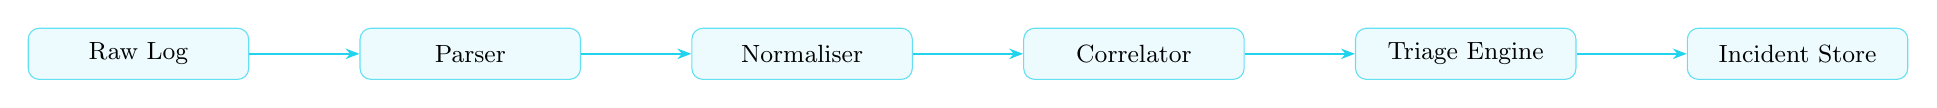
\begin{tikzpicture}[
  stage/.style={rectangle, rounded corners=4pt, draw=siriusblue!70, fill=siriusblue!8,
                minimum width=2.8cm, minimum height=0.65cm, font=\small, text centered},
  arrow/.style={-{Stealth[length=5pt]}, thick, siriusblue}
]
\node[stage] (raw)    {Raw Log};
\node[stage, right=1.4cm of raw]   (parse) {Parser};
\node[stage, right=1.4cm of parse] (norm)  {Normaliser};
\node[stage, right=1.4cm of norm]  (corr)  {Correlator};
\node[stage, right=1.4cm of corr]  (triage){Triage Engine};
\node[stage, right=1.4cm of triage](store) {Incident Store};

\draw[arrow] (raw) -- (parse);
\draw[arrow] (parse) -- (norm);
\draw[arrow] (norm) -- (corr);
\draw[arrow] (corr) -- (triage);
\draw[arrow] (triage) -- (store);
\end{tikzpicture}
\caption{Log ingestion and triage pipeline}
\end{figure}

% =============================================================================
\section{Security Engineering Considerations}
% =============================================================================

\subsection{API Security Controls}

\begin{table}[H]
\centering
\caption{API security measures implemented}
\begin{tabular}{lp{9cm}}
\toprule
\textbf{Control} & \textbf{Implementation} \\
\midrule
CORS             & Strict origin allowlist (\texttt{localhost:5173} only in development) \\
Input validation & Pydantic v2 \texttt{Field} constraints (\texttt{min\_length}, \texttt{ge}, \texttt{le}) \\
Error handling   & Structured JSON error responses; no stack traces exposed \\
Rate limiting    & Not in scope (portfolio); \texttt{slowapi} recommended for production \\
Authentication   & Not in scope (portfolio); OAuth 2.0 / JWT recommended for production \\
\bottomrule
\end{tabular}
\end{table}

\subsection{Agent Safety Constraints}

The security agent is strictly limited to read-only passive reconnaissance:

\begin{itemize}[noitemsep]
  \item All HTTP requests use \texttt{User-Agent: SiriusAI-Agent/2.0} for transparency
  \item 8-second timeout on every network request --- no hanging connections
  \item No write operations, no login attempts, no payload delivery
  \item CVE search uses the public NIST NVD API (no API key required)
  \item Subdomain enumeration is passive (Certificate Transparency, not DNS brute-force)
\end{itemize}

\subsection{Minimal Dependency Philosophy}

\begin{infobox}[title=Standard Library First]
The backend's core features --- agent tools, anomaly detection, SIGMA generation ---
rely exclusively on Python's standard library for all network operations
(\texttt{ssl}, \texttt{socket}, \texttt{urllib}). This eliminates supply-chain risk
from third-party HTTP clients, reduces the attack surface, and makes the codebase
portable across Python 3.10+ environments with no additional package installation.
\end{infobox}

% =============================================================================
\section{Deployment}
% =============================================================================

\subsection{Local Development Setup}

\begin{lstlisting}[style=pythonstyle, caption=Development environment bootstrap]
# --- Backend ---
cd backend
python -m venv .venv && source .venv/bin/activate
pip install -r requirements.txt
uvicorn app.main:app --reload --port 8000

# --- Frontend (separate terminal) ---
cd frontend
npm install
npm run dev          # Vite dev server at http://localhost:5173
\end{lstlisting}

\subsection{Environment Variables}

\begin{table}[H]
\centering
\caption{Backend environment variable reference}
\begin{tabular}{llp{6cm}}
\toprule
\textbf{Variable} & \textbf{Default} & \textbf{Description} \\
\midrule
\texttt{APP\_NAME}        & SIRIUS AI & Application display name \\
\texttt{OPENAI\_API\_KEY} & (empty)   & Enables LLM-powered agent \& copilot \\
\texttt{OPENAI\_BASE\_URL} & (empty)  & Optional base URL for local LLM proxy \\
\texttt{LOG\_LEVEL}       & INFO      & Python logging level \\
\bottomrule
\end{tabular}
\end{table}

\subsection{Python Dependencies}

\begin{table}[H]
\centering
\caption{Backend Python package requirements}
\begin{tabular}{lll}
\toprule
\textbf{Package} & \textbf{Version} & \textbf{Purpose} \\
\midrule
\texttt{fastapi}           & $\geq$ 0.115 & Async web framework \\
\texttt{uvicorn[standard]} & $\geq$ 0.30  & ASGI server \\
\texttt{pydantic-settings} & $\geq$ 2.0   & Config management \\
\midrule
\multicolumn{3}{l}{\textit{Standard library (no pip install required):}} \\
\texttt{ssl}    & stdlib & TLS certificate analysis \\
\texttt{socket} & stdlib & DNS resolution \\
\texttt{urllib} & stdlib & HTTP requests \\
\texttt{json}   & stdlib & Serialisation \\
\texttt{math}   & stdlib & Z-score, RMS calculations \\
\texttt{sqlite3} & stdlib & Pentest session persistence \\
\bottomrule
\end{tabular}
\end{table}

% =============================================================================
\section{Testing}
% =============================================================================

\subsection{Backend Test Suite}

\begin{table}[H]
\centering
\caption{Backend test module inventory}
\begin{tabular}{lp{9cm}}
\toprule
\textbf{Module} & \textbf{Coverage} \\
\midrule
\texttt{test\_api.py}                  & Health check, incident listing, filter endpoints \\
\texttt{test\_incidents\_service.py}   & Enrichment, filtering, pagination logic \\
\texttt{test\_triage\_engine.py}       & Risk scoring, indicator detection, severity mapping \\
\texttt{test\_explanation\_service.py} & LLM and fallback explanation generation \\
\texttt{test\_review\_service.py}      & Analyst review CRUD, status transitions \\
\texttt{test\_upload\_routes.py}       & Log upload, parse, correlation pipeline \\
\bottomrule
\end{tabular}
\end{table}

\subsection{Frontend Type Safety}

TypeScript strict mode is enforced across the entire frontend codebase. Clean compilation
is verified with:

\begin{lstlisting}[style=tsstyle, caption=TypeScript compilation verification]
npx tsc --noEmit    # Zero errors confirmed
\end{lstlisting}

% =============================================================================
\section{Future Roadmap}
% =============================================================================

\begin{enumerate}
  \item \textbf{Production Hardening}
  \begin{itemize}[noitemsep]
    \item JWT / OAuth 2.0 authentication layer
    \item Role-based access control (Tier 1/2/3 analyst roles)
    \item Rate limiting with \texttt{slowapi}
    \item PostgreSQL migration from JSON file store
    \item Kubernetes deployment manifests
  \end{itemize}

  \item \textbf{Detection Engineering}
  \begin{itemize}[noitemsep]
    \item Elasticsearch DSL compilation target
    \item SIGMA rule version control and library management
    \item MITRE Navigator JSON export
    \item Custom rule editor with live preview pane
  \end{itemize}

  \item \textbf{Machine Learning}
  \begin{itemize}[noitemsep]
    \item Replace deterministic baselines with Isolation Forest / LSTM models
    \item Online learning: update baselines from analyst feedback loop
    \item Entity Behaviour Analytics (UEBA) with graph neural networks
    \item Embedding-based similarity search for incident clustering
  \end{itemize}

  \item \textbf{Integrations}
  \begin{itemize}[noitemsep]
    \item Splunk HEC / Microsoft Sentinel API for live log ingestion
    \item JIRA / ServiceNow ticket creation from incidents
    \item Slack / Microsoft Teams alerting for critical findings
    \item VirusTotal and Shodan enrichment in agent tools
  \end{itemize}

  \item \textbf{Agent Enhancements}
  \begin{itemize}[noitemsep]
    \item Port scanning tool (with explicit user consent gate)
    \item Multi-target batch scanning mode
    \item Persistent findings store with trend analysis dashboard
    \item Multi-agent SOC orchestration (specialist sub-agents)
  \end{itemize}
\end{enumerate}

% =============================================================================
\section{Conclusion}
% =============================================================================

SIRIUS AI demonstrates that a lean, modern codebase can deliver capabilities typically
associated with enterprise SOC platforms. By combining industry-standard methodologies
(SIGMA, MITRE ATT\&CK, NIST CSF), real network reconnaissance (Certificate Transparency,
NIST NVD, RDAP), statistical rigour (z-score, RMS composite, risk multipliers), and
modern engineering patterns (ReAct, SSE streaming, Pydantic v2, React 19), the platform
provides a compelling foundation for a production security operations tool.

The architecture is horizontally scalable (stateless FastAPI workers), vertically
extensible (new agent tools, compliance frameworks, and detection modules can be added
without modifying existing code), and vendor-agnostic (SIGMA multi-platform output,
stdlib-only network stack).

\vspace{1.5em}

\begin{techbox}[title=Source Code Repository]
\centering
\href{https://github.com/Karyaustuncelik/AI-Powered-Security-Incident-Triage-Assistant}%
     {https://github.com/Karyaustuncelik/AI-Powered-Security-Incident-Triage-Assistant}
\end{techbox}

% =============================================================================
\appendix
\section{Core Pydantic Model --- EnrichedIncident}
% =============================================================================

\begin{lstlisting}[style=pythonstyle, caption=EnrichedIncident Pydantic model (domain.py)]
class EnrichedIncident(BaseModel):
    incident_id: str
    timestamp:   datetime
    event_type:  IncidentEventType
    category:    IncidentCategory
    affected_entity: str
    actor_user:      str
    source_system:   str
    summary:         str
    technical_facts:     list[TechnicalFact]      = Field(default_factory=list)
    detected_indicators: list[IndicatorType]      = Field(default_factory=list)
    score_breakdown:     list[ScoreContribution]  = Field(default_factory=list)
    score:    int            = Field(..., ge=0, le=100)
    severity: SeverityLevel
    priority: PriorityLevel
    suggested_action: str
    source_event_count:   int = Field(default=0, ge=0)
    source_event_samples: list[str] = Field(default_factory=list)
    review:          IncidentReview     | None = None
    llm_explanation: IncidentExplanation | None = None
\end{lstlisting}

% =============================================================================
\section{SIGMA Rule Field Specification}
% =============================================================================

\begin{table}[H]
\centering
\caption{SIGMA rule fields generated by SIRIUS AI}
\begin{tabular}{lp{9.5cm}}
\toprule
\textbf{Field} & \textbf{Description} \\
\midrule
\texttt{title}         & Human-readable rule name derived from event type \\
\texttt{id}            & UUID v4 unique identifier \\
\texttt{status}        & \texttt{experimental} (new rules) | \texttt{stable} (reviewed) \\
\texttt{description}   & Natural language description of the detection logic \\
\texttt{author}        & \texttt{SIRIUS AI Detection Engine} \\
\texttt{date}          & ISO 8601 generation date \\
\texttt{tags}          & MITRE ATT\&CK tactic slugs + technique IDs \\
\texttt{logsource}     & category / product / service triplet \\
\texttt{detection}     & SIGMA detection block: selection + condition \\
\texttt{level}         & critical | high | medium | low \\
\texttt{falsepositives} & Known benign scenarios to suppress \\
\bottomrule
\end{tabular}
\end{table}

% =============================================================================
\section{Sample Anomaly Detection API Response}
% =============================================================================

\begin{lstlisting}[style=yamlstyle, caption=Full anomaly detection JSON response]
{
  "incident_id": "INC-2026-0042",
  "user_id": "alice@example.com",
  "analysis_timestamp": "2026-05-18T10:23:41Z",
  "is_anomalous": true,
  "composite_z_score": 3.47,
  "risk_multiplier": 1.50,
  "explanation": "Strong anomaly detected across 3 dimensions.",
  "anomaly_scores": [
    {
      "anomaly_type": "login_frequency",
      "z_score": 4.12,
      "observed_value": 23.0,
      "baseline_mean": 5.8,
      "baseline_std": 1.4,
      "is_anomalous": true,
      "is_strong_anomaly": true,
      "description": "23 logins vs baseline of 5.8 (sd=1.4)"
    },
    {
      "anomaly_type": "time_anomaly",
      "z_score": 2.91,
      "observed_value": 1.0,
      "baseline_mean": 0.12,
      "baseline_std": 0.30,
      "is_anomalous": true,
      "is_strong_anomaly": false,
      "description": "After-hours ratio significantly above baseline"
    },
    {
      "anomaly_type": "api_volume",
      "z_score": 1.30,
      "observed_value": 142.0,
      "baseline_mean": 98.5,
      "baseline_std": 33.8,
      "is_anomalous": false,
      "is_strong_anomaly": false,
      "description": "API volume within normal range"
    }
  ]
}
\end{lstlisting}

\end{document}
